% Relatório técnico: pêndulo invertido com roda de reação.
% Todos os números do modelo vêm de valores.tex, gerado por:
%     python -m sim.export_relatorio
% Compilar:  latexmk -pdf relatorio.tex
\documentclass[11pt,a4paper]{article}

\usepackage[utf8]{inputenc}
\usepackage[T1]{fontenc}
\usepackage[brazil]{babel}
\usepackage{lmodern}
\usepackage[a4paper,margin=2.5cm]{geometry}
\usepackage{microtype}
\usepackage{amsmath,amssymb,mathtools,bm,empheq}
\usepackage{siunitx}
\usepackage{booktabs,array,tabularx}
\usepackage{graphicx}
\usepackage{float}
\usepackage{caption,subcaption}
\usepackage{tikz}
\usetikzlibrary{arrows.meta,positioning,calc,shapes.geometric,fit,backgrounds}
\usepackage[hidelinks]{hyperref}

\sisetup{
  output-decimal-marker = {,},
  group-separator = {.},
  group-minimum-digits = 5,
  group-digits = integer,
  exponent-product = \cdot,
  per-mode = symbol,
}
\DeclareSIUnit\rpm{rpm}
\captionsetup{font=small,labelfont=bf}
\graphicspath{{figuras/}}

% ARQUIVO GERADO por sim/export_relatorio.py - não edite à mão.
% Mude sim/params.py e rode: python -m sim.export_relatorio
\newcommand{\vMotorR}{0.8}
\newcommand{\vMotorL}{0.5}
\newcommand{\vMotorNzero}{4000}
\newcommand{\vMotorIzero}{0.6}
\newcommand{\vMotorKe}{0.0275}
\newcommand{\vMotorTauC}{11.6}
\newcommand{\vMotorB}{1.18e-5}
\newcommand{\vMotorBeq}{3.94e-5}
\newcommand{\vMotorMassa}{350}
\newcommand{\vMotorJ}{1e-5}
\newcommand{\vMotorTauEl}{0.62}
\newcommand{\vMotorIpartida}{15}
\newcommand{\vMotorTpartida}{0.413}
\newcommand{\vRodaN}{12}
\newcommand{\vRodaMconj}{24}
\newcommand{\vRodaRparaf}{48}
\newcommand{\vRodaDext}{116}
\newcommand{\vRodaDaleta}{132}
\newcommand{\vRodaMassa}{385}
\newcommand{\vRodaMimpressa}{82}
\newcommand{\vRodaIw}{8.57e-4}
\newcommand{\vRodaRanhuras}{40}
\newcommand{\vRodaCpr}{160}
\newcommand{\vRodaEsp}{12}
\newcommand{\vRodaForcaParaf}{51}
\newcommand{\vRodaFracParaf}{77}
\newcommand{\vLw}{96}
\newcommand{\vMbraco}{90}
\newcommand{\vFracCm}{0.25}
\newcommand{\vMextras}{30}
\newcommand{\vLextras}{30}
\newcommand{\vJ}{0.00715}
\newcommand{\vMgl}{0.722}
\newcommand{\vMassaTotal}{855}
\newcommand{\vBp}{5e-4}
\newcommand{\vPoloInst}{10}
\newcommand{\vTqueda}{100}
\newcommand{\vVbus}{12}
\newcommand{\vUmax}{11.4}
\newcommand{\vImax}{10}
\newcommand{\vWmax}{209}
\newcommand{\vWmaxRpm}{2000}
\newcommand{\vTs}{1}
\newcommand{\vFs}{1000}
\newcommand{\vTauMax}{0.275}
\newcommand{\vThetaEst}{22.4}
\newcommand{\vThetaMax}{19.8}
\newcommand{\vHmax}{0.18}
\newcommand{\vCoefC}{9.85e-4}
\newcommand{\vCoefG}{0.0344}
\newcommand{\vPostoCtrb}{3}
\newcommand{\vDesvTheta}{3}
\newcommand{\vDesvThetaDot}{0.5}
\newcommand{\vDesvOmega}{50}
\newcommand{\vDesvU}{11.4}
\newcommand{\vKum}{-248.9}
\newcommand{\vKdois}{-25.85}
\newcommand{\vKtres}{-0.2451}
\newcommand{\vKumGrau}{4.34}
\newcommand{\vKtresRpm}{-2.57}
\newcommand{\vRaioEspectral}{0.99912}
\newcommand{\vEixoFora}{18.1}
\newcommand{\vDistSensores}{12.2}
\newcommand{\vBarraComp}{82}
\newcommand{\vYroda}{8}
\newcommand{\vAnguloBatente}{25}
\newcommand{\vHpivo}{50}
\newcommand{\vCauda}{40}
\newcommand{\vCadRodaMassa}{73}
\newcommand{\vCadRodaVol}{68.1}
\newcommand{\vCadRodaDim}{132 \times 132 \times 12}
\newcommand{\vCadBracoMassa}{53}
\newcommand{\vCadBracoVol}{55.5}
\newcommand{\vCadBracoDim}{56 \times 164 \times 34}
\newcommand{\vCadSuporteSensoresMassa}{11}
\newcommand{\vCadSuporteSensoresVol}{10}
\newcommand{\vCadSuporteSensoresDim}{76 \times 28 \times 20}
\newcommand{\vCadBaseMassa}{190}
\newcommand{\vCadBaseVol}{332}
\newcommand{\vCadBaseDim}{170 \times 185 \times 67}
\newcommand{\vCadBandejaMassa}{20}
\newcommand{\vCadBandejaVol}{26.8}
\newcommand{\vCadBandejaDim}{150 \times 66 \times 3}
\newcommand{\vCadBatenteTpuMassa}{2.2}
\newcommand{\vCadBatenteTpuVol}{1.81}
\newcommand{\vCadBatenteTpuDim}{38 \times 16 \times 3}
\newcommand{\vCadRodaInercia}{1.65e-4}
\newcommand{\matA}{\begin{bmatrix} \num{0} & \num{1} & \num{0} \\ \num{100.9} & \num{-0.06991} & \num{0.1377} \\ \num{-100.9} & \num{0.06991} & \num{-1.286} \end{bmatrix}}
\newcommand{\matB}{\begin{bmatrix} \num{0} \\ \num{-4.806} \\ \num{44.9} \end{bmatrix}}
\newcommand{\matAd}{\begin{bmatrix} \num{1.0001} & \num{9.9998e-4} & \num{6.8817e-8} \\ \num{0.10094} & \num{0.99998} & \num{1.376e-4} \\ \num{-0.10088} & \num{1.941e-5} & \num{0.99871} \end{bmatrix}}
\newcommand{\matBd}{\begin{bmatrix} \num{-2.4e-6} \\ \num{-0.0048} \\ \num{0.0449} \end{bmatrix}}
\newcommand{\matCtrb}{\begin{bmatrix} \num{0} & \num{-4.81} & \num{6.52} \\ \num{-4.81} & \num{6.52} & \num{-494} \\ \num{44.9} & \num{-58.1} & \num{560} \end{bmatrix}}
\newcommand{\matQ}{\begin{bmatrix} \num{365} & \num{0} & \num{0} \\ \num{0} & \num{4} & \num{0} \\ \num{0} & \num{0} & \num{4e-4} \end{bmatrix}}
\newcommand{\matR}{\num{0.00769}}
\newcommand{\matP}{\begin{bmatrix} \num{46800} & \num{876} & \num{48.6} \\ \num{876} & \num{93.5} & \num{5.11} \\ \num{48.6} & \num{5.11} & \num{0.502} \end{bmatrix}}
\newcommand{\matK}{\begin{bmatrix} \num{-248.9} & \num{-25.85} & \num{-0.2451} \end{bmatrix}}
\newcommand{\polosMA}{\num{-10.2}, \num{-1.15} \text{ e } \num{9.95}}
\newcommand{\polosMFz}{\num{0.89537}, \num{0.9905} \text{ e } \num{0.99912}}
\newcommand{\polosMFs}{\num{-111}, \num{-9.55} \text{ e } \num{-0.881}}
\newcommand{\tabelaPinos}{%
\texttt{PB0} & IBT-2 RPWM & TIM3\_CH3, PWM 20 kHz \\
\texttt{PB1} & IBT-2 LPWM & TIM3\_CH4, PWM 20 kHz \\
\texttt{PB10} & IBT-2 R\_EN + L\_EN (juntos) & GPIO, pull-down externo 10 k \\
\texttt{PA15} & Sensor óptico A (D0) & TIM2\_CH1, modo encoder \\
\texttt{PB3} & Sensor óptico B (D0) & TIM2\_CH2, modo encoder \\
\texttt{PB6} & MPU6050 SCL & I2C1, 400 kHz \\
\texttt{PB7} & MPU6050 SDA & I2C1 \\
\texttt{PA2} & Telemetria TX ($\to$ RX do adaptador USB-serial) & USART2 \\
\texttt{PA3} & Telemetria RX ($\leftarrow$ TX do adaptador USB-serial) & USART2 \\
\texttt{PA4} & Tensão do barramento (divisor 10 k / 2,2 k) & ADC1\_IN4 \\
\texttt{PA5} & IBT-2 R\_IS (divisor 10 k / 10 k, opcional) & ADC1\_IN5 \\
\texttt{PA6} & IBT-2 L\_IS (divisor 10 k / 10 k, opcional) & ADC1\_IN6 \\
\texttt{PA0} & Botão KEY da placa (armar / parar) & GPIO, ativo em nível baixo \\
\texttt{PC13} & LED da placa & GPIO, ativo em nível baixo \\
}


% notação
\newcommand{\dd}{\mathrm{d}}
\newcommand{\vt}[1]{\bm{#1}}
\newcommand{\xref}{\vt{x}_{\mathrm{r}}}

\title{\textbf{Pêndulo invertido com roda de reação}\\[4pt]
  \large Modelagem por Euler-Lagrange e controle LQR em variáveis de erro}
\author{}
\date{Trabalho de SEC \\[2pt] Novembro de 2026}

\begin{document}
\maketitle

\begin{abstract}
\noindent
Este relatório descreve o projeto de um pêndulo invertido estabilizado por uma roda de
reação, controlado por uma placa WeAct Black Pill (STM32F411CEU6). O modelo dinâmico é
deduzido pelo formalismo de Euler-Lagrange, com duas coordenadas generalizadas (ângulo
do braço e ângulo da roda) e o motor de corrente contínua acoplado como força generalizada.
O modelo é linearizado em torno do equilíbrio e reescrito em variáveis de erro, sobre as
quais se projeta um regulador linear quadrático (LQR) discreto a \qty{\vFs}{\hertz}.
Com os parâmetros estimados, o controlador recupera o pêndulo solto de até
\qty{\vThetaMax}{\degree} da vertical, perto do limite físico de
\qty{\vThetaEst}{\degree} imposto pelo torque máximo do motor. O relatório também
apresenta o dimensionamento da roda, as peças mecânicas e o hardware.
\end{abstract}

\tableofcontents
\newpage

% =====================================================================
\section{Introdução}

O pêndulo invertido é um problema clássico de controle: o equilíbrio na vertical é
instável e qualquer perturbação faz o braço cair em uma fração de segundo. Na versão
com roda de reação, não há carrinho nem base móvel. Um motor preso no topo do braço
acelera uma roda pesada, e o torque de reação que a roda aplica no motor (e, portanto,
no braço) é o único meio de atuação. Acelerar a roda num sentido empurra o braço no
sentido oposto.

O sistema tem uma característica que o torna mais interessante que um pêndulo comum:
a roda não pode acelerar para sempre, porque sua velocidade é limitada pelo motor. O
controlador precisa, ao mesmo tempo, manter o braço em pé e trazer a roda de volta ao
repouso, e a única forma de tirar momento angular da roda é inclinar o braço e deixar
a gravidade agir (Seção~\ref{sec:interpretacao}).

O projeto completo (simulação, firmware, peças mecânicas e documentação) foi feito de
forma que todos os números deste relatório saiam de um único arquivo de parâmetros
(\texttt{sim/params.py}), garantindo que modelo, firmware e peças estejam coerentes.

% =====================================================================
\section{Descrição do sistema}

A Figura~\ref{fig:blocos} mostra a arquitetura. Um sensor inercial MPU6050 preso no braço
mede o ângulo (pelo acelerômetro) e a velocidade angular (pelo giroscópio). Dois sensores
ópticos de fenda leem um anel dentado de \vRodaRanhuras{} dentes na borda da roda e
formam um encoder em quadratura de \vRodaCpr{} contagens por volta. A Black Pill executa
a malha de controle a \qty{\vFs}{\hertz} e comanda a ponte H BTS7960 por PWM de
\qty{20}{\kilo\hertz}, que alimenta o motor 775 a partir de uma fonte de \qty{\vVbus}{\volt}.

\begin{figure}[H]
\centering
\begin{tikzpicture}[
  bloco/.style={draw, rounded corners=2pt, align=center, minimum height=11mm, minimum width=27mm, font=\small, fill=white},
  seta/.style={-{Latex[length=2.2mm]}, thick},
  fis/.style={-{Latex[length=2.2mm]}, thick, dashed, gray!70!black},
  rot/.style={font=\scriptsize, midway, fill=white, inner sep=1pt},
  node distance=9mm and 14mm]
  \node[bloco, fill=blue!6] (bp) {Black Pill\\STM32F411\\controle a \qty{\vFs}{\hertz}};
  \node[bloco, above left=4mm and 16mm of bp] (mpu) {MPU6050\\acelerômetro + giroscópio};
  \node[bloco, below left=4mm and 16mm of bp] (enc) {2 sensores ópticos\\encoder \vRodaCpr{} cont./volta};
  \node[bloco, right=14mm of bp] (ibt) {Ponte H\\BTS7960 (IBT-2)};
  \node[bloco, right=12mm of ibt] (mot) {Motor 775\\+ roda de reação};
  \node[bloco, below=12mm of mot, fill=orange!8] (pend) {Pêndulo\\$\theta$, $\dot\theta$, $\omega$};
  \node[bloco, above=9mm of ibt] (fonte) {Fonte \qty{\vVbus}{\volt}\\+ fusível};
  \node[bloco, below=10mm of bp] (ser) {Adaptador USB-serial\\telemetria e comandos};
  \draw[seta] (mpu) -- node[rot]{I2C \qty{400}{\kilo\hertz}} (bp);
  \draw[seta] (enc) -- node[rot]{TIM2 quadratura} (bp);
  \draw[seta] (bp) -- node[rot]{PWM} (ibt);
  \draw[seta] (ibt) -- node[rot]{\qty{0}{}--\qty{\vVbus}{\volt}} (mot);
  \draw[seta] (fonte) -- (ibt);
  \draw[seta] (fonte.west) -| node[rot, pos=0.25]{buck \qty{5}{\volt}} (bp.north);
  \draw[seta, <->] (bp) -- node[rot]{UART} (ser);
  \draw[fis] (mot) -- node[rot]{torque de reação} (pend);
  \draw[fis] (pend.south) |- ++(0,-6mm) -| ($(enc.south)+(0,0)$) node[pos=0.25, font=\scriptsize, below]{giro da roda};
  \draw[fis] (pend.east) -- ++(6mm,0) |- ($(mpu.north)+(0,6mm)$) -- (mpu.north) node[pos=0.0, font=\scriptsize, above, xshift=30mm]{inclinação do braço};
\end{tikzpicture}
\caption{Arquitetura do sistema. Setas cheias: sinais elétricos; tracejadas: acoplamento físico.}
\label{fig:blocos}
\end{figure}

% =====================================================================
\section{Modelagem por Euler-Lagrange}
\label{sec:lagrange}

\subsection{Coordenadas generalizadas e hipóteses}

O sistema tem dois graus de liberdade (Figura~\ref{fig:esquema}):
\begin{itemize}
  \item $\theta$: ângulo do braço medido a partir da vertical para cima;
  \item $\varphi$: ângulo da roda \emph{em relação ao braço}, que é o que o encoder mede.
        A velocidade relativa é $\omega = \dot\varphi$.
\end{itemize}
Os dois ângulos são medidos no mesmo sentido de rotação, de modo que a velocidade
angular absoluta da roda é $\dot\theta + \dot\varphi$. Hipóteses: corpos rígidos;
pivô e eixo do motor paralelos; roda balanceada (centro de massa no eixo do motor);
atrito viscoso no pivô; atrito seco e viscoso no motor.

\begin{figure}[H]
\centering
\begin{tikzpicture}[scale=1.0, >={Latex[length=2.2mm]}]
  \def\th{18}
  \def\L{4.4}
  \coordinate (O) at (0,0);
  \coordinate (W) at ({\L*sin(\th)},{\L*cos(\th)});
  \coordinate (Bc) at ({0.2*\L*sin(\th)},{0.2*\L*cos(\th)});
  \coordinate (A) at ({0.43*\L*sin(\th)},{0.43*\L*cos(\th)});
  % base e pivô
  \fill[gray!25] (-2.4,-0.55) rectangle (2.8,-0.35);
  \draw[thick] (-2.4,-0.35) -- (2.8,-0.35);
  \draw[thick, fill=gray!15] (-0.35,-0.35) -- (0,0) -- (0.35,-0.35);
  % vertical de referência
  \draw[dashed, gray] (O) -- (0,\L+1.9);
  % braço
  \draw[line width=4pt, blue!45!black, line cap=round] (O) -- (W);
  \fill[white] (O) circle (0.09); \draw (O) circle (0.09);
  % roda
  \draw[thick, orange!80!black, fill=orange!12] (W) circle (1.35);
  \foreach \a in {0,60,...,300} \draw[orange!70!black, thick] (W) -- ++({\a+15}:1.0);
  \foreach \a in {0,30,...,330} \fill[gray!60] (W) ++({\a+7}:1.12) circle (0.08);
  \fill[blue!45!black] (W) circle (0.12);
  % ângulo theta
  \draw[->, thick] (0,1.1) arc[start angle=90, end angle={90-\th}, radius=1.1];
  \node at ({1.4*sin(\th/2)},{1.4*cos(\th/2)}) {$\theta$};
  % phi e tau na roda (sentido horário = positivo)
  \draw[->, very thick, red!70!black] ($(W)+(125:1.7)$) arc[start angle=125, end angle=45, radius=1.7];
  \node[red!70!black, right] at ($(W)+(50:1.8)$) {$\varphi,\ \tau$ (na roda)};
  % reação no braço (sentido anti-horário)
  \draw[->, thick, red!70!black] ($(A)+(-60:0.45)$) arc[start angle=-60, end angle=60, radius=0.45];
  \node[red!70!black, right] at ($(A)+(0.45,0)$) {$-\tau$ (no braço)};
  % comprimento, paralelo ao braço e deslocado para a esquerda
  \draw[|<->|, gray!60!black] ($(O)!0.65cm!90:(W)$) -- ($(W)!0.65cm!-90:(O)$)
     node[midway, left, black] {$l_w$};
  % pesos
  \draw[->, thick] (W) -- ++(0,-1.75) node[right, font=\small] {$(m_m + m_w)\,g$};
  \fill (Bc) circle (0.06);
  \draw[->, thick] (Bc) -- ++(0,-0.6) node[right, font=\small] {$m_b\,g$};
  % rótulos
  \node[font=\small, below] at (0,-0.6) {pivô (rolamentos 608)};
\end{tikzpicture}
\caption{Coordenadas generalizadas. O motor aplica o torque $\tau$ na roda e, pela terceira
lei de Newton, $-\tau$ no braço; os dois ângulos são positivos no mesmo sentido.}
\label{fig:esquema}
\end{figure}

\subsection{Energias e Lagrangiano}

Seja $J$ o momento de inércia de todo o conjunto em torno do pivô, \emph{sem} incluir o
giro da roda em torno do próprio eixo (motor e roda tratados como massas no fim do braço,
mais o braço e os componentes), e $I_w$ o momento de inércia da roda e do rotor do motor
em torno do eixo do motor:
\begin{equation}
  J = (m_m + m_w)\,l_w^2 + \tfrac12 m_m r_m^2 + \tfrac13 m_b l_w^2 + m_e l_e^2 ,
  \qquad
  I_w = I_{\text{roda}} + J_{\text{rotor}} .
\end{equation}
A energia cinética soma a rotação do conjunto em torno do pivô e a rotação absoluta
da roda:
\begin{equation}
  T = \tfrac12 J\,\dot\theta^2 + \tfrac12 I_w\,(\dot\theta + \dot\varphi)^2 .
  \label{eq:T}
\end{equation}
Com o pivô como referência, a energia potencial gravitacional é
\begin{equation}
  V = Mgl\,\cos\theta ,
  \qquad
  Mgl = g\,\bigl[(m_m + m_w)\,l_w + m_b\,l_{cb} + m_e\,l_e\bigr] ,
  \label{eq:V}
\end{equation}
em que $l_{cb}$ é a altura do centro de massa do braço. O Lagrangiano é
\begin{equation}
  \mathcal{L} = T - V
  = \tfrac12 J\,\dot\theta^2 + \tfrac12 I_w\,(\dot\theta + \dot\varphi)^2 - Mgl\,\cos\theta .
\end{equation}

\subsection{Forças generalizadas}

As forças não conservativas entram pelo trabalho virtual. O motor aplica $+\tau$ na roda
e $-\tau$ no braço; com deslocamentos virtuais $\delta\theta$ e $\delta\varphi$, a roda gira
$\delta\theta + \delta\varphi$ e o braço gira $\delta\theta$:
\begin{equation}
  \delta W = \tau\,(\delta\theta + \delta\varphi) - \tau\,\delta\theta - b_p\,\dot\theta\,\delta\theta
           = \underbrace{\bigl(-b_p\,\dot\theta\bigr)}_{Q_\theta}\,\delta\theta
           + \underbrace{\tau}_{Q_\varphi}\,\delta\varphi .
\end{equation}
O torque do motor é \emph{interno} ao conjunto: ele não aparece na equação de $\theta$, só na
de $\varphi$. O torque líquido $\tau$ é o torque eletromagnético menos o atrito do motor:
\begin{equation}
  \tau = k_t\, i - \tau_{\text{at}}(\omega),
  \qquad
  \tau_{\text{at}}(\omega) = \tau_c \tanh(\omega/\varepsilon) + b\,\omega ,
  \label{eq:tau}
\end{equation}
em que a tangente hiperbólica é uma versão suave do atrito seco das escovas.

\subsection{Equações de Euler-Lagrange}

Para cada coordenada, $\dfrac{\dd}{\dd t}\dfrac{\partial\mathcal{L}}{\partial\dot q}
- \dfrac{\partial\mathcal{L}}{\partial q} = Q_q$. As derivadas parciais são
\begin{align}
  \frac{\partial\mathcal{L}}{\partial\dot\theta} &= J\dot\theta + I_w(\dot\theta + \dot\varphi), &
  \frac{\partial\mathcal{L}}{\partial\theta} &= Mgl\,\sin\theta, \\
  \frac{\partial\mathcal{L}}{\partial\dot\varphi} &= I_w(\dot\theta + \dot\varphi), &
  \frac{\partial\mathcal{L}}{\partial\varphi} &= 0 .
\end{align}
Logo:
\begin{align}
  \text{em } \theta:&\quad (J + I_w)\,\ddot\theta + I_w\,\ddot\varphi - Mgl\,\sin\theta = -b_p\,\dot\theta,
  \label{eq:el1}\\
  \text{em } \varphi:&\quad I_w\,(\ddot\theta + \ddot\varphi) = \tau .
  \label{eq:el2}
\end{align}
Subtraindo \eqref{eq:el2} de \eqref{eq:el1}, o termo de $I_w$ some e fica a equação do braço;
voltando em \eqref{eq:el2}, sai a da roda:
\begin{empheq}[box=\fbox]{align}
  J\,\ddot\theta &= Mgl\,\sin\theta - b_p\,\dot\theta - \tau ,
  \label{eq:braco}\\
  \dot\omega = \ddot\varphi &= \frac{\tau}{I_w} - \ddot\theta
  = \Bigl(\frac{1}{I_w} + \frac{1}{J}\Bigr)\tau - \frac{Mgl\,\sin\theta - b_p\,\dot\theta}{J} .
  \label{eq:roda}
\end{empheq}
A Equação~\eqref{eq:braco} mostra o princípio da roda de reação: o braço sente $-\tau$.
Essas mesmas equações foram deduzidas simbolicamente com o SymPy
(\texttt{sim/derivacao.py}) e conferidas, ponto a ponto, contra o modelo numérico da simulação.

\subsection{Motor de corrente contínua}

O circuito de armadura obedece a
\begin{equation}
  L\,\frac{\dd i}{\dd t} = u - R\,i - k_e\,\omega ,
\end{equation}
com $u$ a tensão média aplicada pela ponte H e $k_e = k_t$ em unidades SI. A constante de
tempo elétrica $L/R \approx \qty{\vMotorTauEl}{\milli\second}$ é muito menor que a escala de
tempo da queda do pêndulo ($1/\sqrt{Mgl/J} \approx \qty{\vTqueda}{\milli\second}$), então no
modelo de projeto a corrente é tomada em regime, $i = (u - k_e\,\omega)/R$, e o torque fica
\begin{equation}
  \tau = \frac{k_t}{R}\,u - \frac{k_t k_e}{R}\,\omega - \tau_{\text{at}}(\omega) .
  \label{eq:tau_u}
\end{equation}
O termo $k_t k_e\,\omega/R$ é o freio da força contraeletromotriz: quanto mais rápido a roda
gira, menos torque a mesma tensão produz. A simulação de validação mantém a indutância.

\subsection{Modelo não linear em espaço de estados}

Com o estado $\vt{x} = \begin{bmatrix}\theta & \dot\theta & \omega\end{bmatrix}^{\!\top}$ e a
entrada $u$ (tensão do motor), as Equações~\eqref{eq:braco}--\eqref{eq:tau_u} dão
\begin{equation}
  \dot{\vt{x}} = \vt{f}(\vt{x}, u) =
  \begin{bmatrix}
    \dot\theta \\[2pt]
    \dfrac{Mgl\sin\theta - b_p\dot\theta - \tau(u,\omega)}{J} \\[10pt]
    \Bigl(\dfrac{1}{I_w} + \dfrac{1}{J}\Bigr)\tau(u,\omega) - \dfrac{Mgl\sin\theta - b_p\dot\theta}{J}
  \end{bmatrix} .
  \label{eq:naolinear}
\end{equation}
O ângulo absoluto da roda não aparece: o sistema não depende de $\varphi$, só de $\omega$.

\subsection{Verificações físicas do modelo}

Duas propriedades decorrem diretamente das Equações~\eqref{eq:el1}--\eqref{eq:el2} e servem
de teste para qualquer implementação:
\begin{itemize}
  \item \textbf{Momento angular.} Com $H = \partial\mathcal{L}/\partial\dot\theta
    = J\dot\theta + I_w(\dot\theta + \dot\varphi)$, a Equação~\eqref{eq:el1} dá
    \begin{equation}
      \dot H = Mgl\,\sin\theta - b_p\,\dot\theta .
      \label{eq:momento}
    \end{equation}
    O motor não altera o momento angular total: só a gravidade e o atrito do pivô o fazem.
  \item \textbf{Energia.} Sem motor e sem atrito, $E = T + V$ é constante.
\end{itemize}
As duas propriedades são verificadas numericamente na suíte de testes do projeto
(\texttt{sim/tests/test\_modelo.py}).

% =====================================================================
\section{Linearização e modelo de erro}
\label{sec:erro}

\subsection{Equilíbrios}

Fazendo $\dot{\vt{x}} = 0$ em \eqref{eq:naolinear}: $\dot\theta = 0$ e, da terceira linha
somada à segunda, $\tau = 0$; daí $\sin\theta = 0$. Para o atrito linearizado, $\tau = 0$
admite qualquer velocidade constante da roda desde que a tensão compense a força
contraeletromotriz e o atrito. Os equilíbrios do braço em pé formam a família
\begin{equation}
  \xref = \begin{bmatrix}\theta_{\mathrm{eq}} & 0 & \omega_{\mathrm{r}}\end{bmatrix}^{\!\top},
  \qquad
  u_{\mathrm{r}} = \Bigl(k_e + \frac{R\,b_{\text{eq}}}{k_t}\Bigr)\,\omega_{\mathrm{r}} ,
\end{equation}
em que $\theta_{\mathrm{eq}}$ é o ângulo, \emph{na referência do sensor}, em que o centro de massa
fica exatamente acima do pivô. Idealmente $\theta_{\mathrm{eq}} = 0$, mas um MPU6050 montado
levemente torto, ou um centro de massa fora do eixo do braço, deslocam esse valor. O objetivo
de controle é o braço em pé com a roda parada: $\omega_{\mathrm{r}} = 0$, $u_{\mathrm{r}} = 0$.

\subsection{Variáveis de erro}

Define-se o erro em relação ao equilíbrio desejado e o desvio da entrada:
\begin{equation}
  \vt{e} = \vt{x} - \xref =
  \begin{bmatrix} \theta - \theta_{\mathrm{eq}} \\ \dot\theta \\ \omega - \omega_{\mathrm{r}} \end{bmatrix},
  \qquad
  \tilde u = u - u_{\mathrm{r}} .
\end{equation}
Como $\vt{f}(\xref, u_{\mathrm{r}}) = 0$, a expansão de Taylor de primeira ordem dá a
dinâmica do erro
\begin{equation}
  \dot{\vt{e}} = A\,\vt{e} + B\,\tilde u ,
  \qquad
  A = \left.\frac{\partial\vt{f}}{\partial\vt{x}}\right|_{\xref,\,u_{\mathrm{r}}},
  \quad
  B = \left.\frac{\partial\vt{f}}{\partial u}\right|_{\xref,\,u_{\mathrm{r}}} .
  \label{eq:erro}
\end{equation}
A aproximação usada é $\sin\theta \approx \theta$, com erro relativo abaixo de \qty{1}{\percent}
até \qty{14}{\degree}. O atrito do motor é substituído pela secante na rotação em vazio,
$b_{\text{eq}} = \tau_{\text{at}}(\omega_0)/\omega_0$, porque a derivada da parcela de atrito
seco na origem não representa o comportamento médio. Com
\begin{equation}
  g_u = \frac{k_t}{R} = \qty{\vCoefG}{\newton\metre\per\volt},
  \qquad
  c = \frac{k_t k_e}{R} + b_{\text{eq}} = \qty{\vCoefC}{\newton\metre\second\per\radian},
\end{equation}
o torque linearizado é $\tau \approx g_u\,\tilde u - c\,(\omega - \omega_{\mathrm{r}})$, e as matrizes ficam
\begin{equation}
  A =
  \begin{bmatrix}
    0 & 1 & 0 \\[2pt]
    \dfrac{Mgl}{J} & -\dfrac{b_p}{J} & \dfrac{c}{J} \\[8pt]
    -\dfrac{Mgl}{J} & \dfrac{b_p}{J} & -c\Bigl(\dfrac{1}{I_w} + \dfrac{1}{J}\Bigr)
  \end{bmatrix},
  \qquad
  B =
  \begin{bmatrix}
    0 \\[2pt] -\dfrac{g_u}{J} \\[8pt] g_u\Bigl(\dfrac{1}{I_w} + \dfrac{1}{J}\Bigr)
  \end{bmatrix} .
\end{equation}
Com os parâmetros do Apêndice~\ref{ap:parametros}:
\begin{equation}
  A = \matA ,
  \qquad
  B = \matB .
\end{equation}

\subsection{Estabilidade em malha aberta e controlabilidade}

Os autovalores de $A$ são $\polosMA$~\unit{\radian\per\second}. O polo positivo,
próximo de $\sqrt{Mgl/J} = \qty{\vPoloInst}{\per\second}$, é a queda do pêndulo: sem controle,
um erro inicial é multiplicado por $e$ a cada \qty{\vTqueda}{\milli\second}. A matriz de
controlabilidade
\begin{equation}
  \mathcal{C} = \begin{bmatrix} B & AB & A^2B \end{bmatrix} = \matCtrb
\end{equation}
tem posto \vPostoCtrb, igual à ordem do sistema: todos os estados do erro podem ser levados a
zero pela tensão do motor.

\subsection{Discretização}

O controle roda a cada $T_s = \qty{\vTs}{\milli\second}$ e a tensão é mantida constante
entre amostras (segurador de ordem zero). O modelo discreto exato é
\begin{equation}
  \vt{e}_{k+1} = A_d\,\vt{e}_k + B_d\,\tilde u_k ,
  \qquad
  A_d = e^{A T_s},
  \qquad
  B_d = \int_0^{T_s} e^{A\eta}\,\dd\eta\; B ,
\end{equation}
\begin{equation}
  A_d = \matAd ,
  \qquad
  B_d = \matBd .
\end{equation}
O primeiro elemento de $A_d$, maior que 1, é a assinatura discreta da instabilidade.

% =====================================================================
\section{Controle LQR em variáveis de erro}
\label{sec:lqr}

\subsection{Problema de otimização}

O LQR escolhe a sequência de tensões que minimiza
\begin{equation}
  \mathcal{J} = \sum_{k=0}^{\infty} \Bigl( \vt{e}_k^{\top} Q\, \vt{e}_k + \tilde u_k^{\top} R\, \tilde u_k \Bigr),
  \qquad Q \succeq 0,\ R \succ 0 ,
\end{equation}
sujeito a $\vt{e}_{k+1} = A_d\vt{e}_k + B_d\tilde u_k$. Os pesos seguem a regra de Bryson: cada
termo é dividido pelo quadrado do maior valor aceitável da variável, o que deixa as parcelas
adimensionais e comparáveis:
\begin{equation}
  Q = \operatorname{diag}\!\Bigl(\frac{1}{\theta_{\max}^2},\ \frac{1}{\dot\theta_{\max}^2},\ \frac{1}{\omega_{\max}^2}\Bigr),
  \qquad
  R = \frac{1}{u_{\max}^2},
\end{equation}
com $\theta_{\max} = \qty{\vDesvTheta}{\degree}$, $\dot\theta_{\max} = \qty{\vDesvThetaDot}{\radian\per\second}$,
$\omega_{\max} = \qty{\vDesvOmega}{\radian\per\second}$ e $u_{\max} = \qty{\vDesvU}{\volt}$:
\begin{equation}
  Q = \matQ ,
  \qquad
  R = \matR .
\end{equation}
O peso pequeno em $\omega$ diz que a roda pode girar à vontade durante uma correção, desde que
volte ao repouso depois; o peso grande em $\theta$ diz que o braço deve ficar muito perto da vertical.

\subsection{Solução: equação de Riccati}

A solução ótima é uma realimentação linear do erro, $\tilde u_k = -K\,\vt{e}_k$, com
\begin{equation}
  K = \bigl(R + B_d^{\top} P B_d\bigr)^{-1} B_d^{\top} P A_d ,
\end{equation}
em que $P$ é a solução simétrica positiva definida da equação algébrica de Riccati discreta
\begin{equation}
  P = A_d^{\top} P A_d - A_d^{\top} P B_d \bigl(R + B_d^{\top} P B_d\bigr)^{-1} B_d^{\top} P A_d + Q .
\end{equation}
Numericamente:
\begin{equation}
  P = \matP ,
  \qquad
  K = \matK .
\end{equation}
A lei de controle, nas variáveis originais, é
\begin{equation}
  \boxed{\;u = u_{\mathrm{r}} - K\,(\vt{x} - \xref)
  = -K_1\,(\theta - \theta_{\mathrm{eq}}) - K_2\,\dot\theta - K_3\,\omega\;}
  \qquad (\omega_{\mathrm{r}} = 0).
\end{equation}

\subsection{Malha fechada}

Os autovalores de $A_d - B_d K$ são $\polosMFz$, todos dentro do círculo unitário (raio
espectral \num{\vRaioEspectral}). Os polos contínuos equivalentes, $s = \ln z / T_s$, são
$\polosMFs$~\unit{\per\second}:
\begin{itemize}
  \item o polo rápido corresponde à rigidez do ângulo, limitada pela tensão e pela corrente
    disponíveis;
  \item o polo intermediário é praticamente o espelho do polo instável de malha aberta,
    comportamento típico do LQR quando o esforço de controle tem custo;
  \item o polo lento é a volta da roda ao repouso, com constante de tempo próxima de
    \qty{1}{\second}, coerente com o peso pequeno em $\omega$.
\end{itemize}

\subsection{Interpretação dos ganhos}
\label{sec:interpretacao}

Com $K_1 = \qty{\vKum}{\volt\per\radian}$, cada grau de inclinação pede cerca de
\qty{\vKumGrau}{\volt} no motor. Como $K_1 < 0$, se o braço tomba no sentido positivo a lei
aplica tensão positiva, a roda acelera no sentido positivo e a reação ($-\tau$) empurra o
braço de volta. $K_2$ é o amortecimento dessa correção.

O sinal de $K_3$ é contraintuitivo: com $K_3 < 0$, a lei aplica \emph{mais} tensão no sentido
em que a roda já gira. A explicação está na Equação~\eqref{eq:momento}: o motor não muda o
momento angular total, só a gravidade muda. Para frear a roda, o controlador precisa primeiro
inclinar o braço levemente, de modo que $Mgl\sin\theta$ retire o momento angular acumulado; e
inclinar o braço nesse sentido exige, momentaneamente, acelerar a roda um pouco mais. O LQR
encontra essa manobra sozinho.

\subsection{Limites físicos e saturação}

A tensão calculada passa por dois limites antes de ir para o PWM. Primeiro, o limite de
corrente, usando o próprio modelo do motor ($i = (u - k_e\omega)/R$):
\begin{equation}
  u \leftarrow \operatorname{sat}\bigl(u,\ k_e\omega - R\,i_{\max},\ k_e\omega + R\,i_{\max}\bigr),
  \qquad i_{\max} = \qty{\vImax}{\ampere};
\end{equation}
depois, o limite de tensão, $|u| \le \qty{\vUmax}{\volt}$ (\qty{95}{\percent} do barramento). Com
isso, o torque máximo é $\tau_{\max} = k_t\,\min(i_{\max}, u_{\max}/R) = \qty{\vTauMax}{\newton\metre}$,
e nenhum controlador consegue segurar o braço parado além de
\begin{equation}
  \theta_{\text{estático}} = \arcsin\frac{\tau_{\max}}{Mgl} = \qty{\vThetaEst}{\degree} .
\end{equation}
Por simulação do modelo não linear \eqref{eq:naolinear} com saturação, o LQR projetado recupera
o pêndulo solto em repouso de até \qty{\vThetaMax}{\degree}, perto desse limite teórico.

\begin{figure}[H]
\centering
\begin{tikzpicture}[
  bloco/.style={draw, rounded corners=2pt, align=center, minimum height=10mm, font=\small, fill=white},
  soma/.style={draw, circle, minimum size=6mm, inner sep=0pt},
  seta/.style={-{Latex[length=2.2mm]}, thick},
  node distance=8mm]
  \node (ref) {$\xref$};
  \node[soma, right=8mm of ref] (s) {};
  \node[font=\scriptsize] at ($(s)+(-0.42,0.25)$) {$+$};
  \node[font=\scriptsize] at ($(s)+(0.25,-0.42)$) {$-$};
  \node[bloco, right=11mm of s] (k) {$-K$};
  \node[bloco, right=10mm of k] (sat) {limite de\\corrente e tensão};
  \node[bloco, right=10mm of sat, fill=orange!8] (pl) {planta não linear\\Eq.~\eqref{eq:naolinear}};
  \node[bloco, below=9mm of sat, fill=blue!6] (est) {estimadores: filtro complementar\\e velocidade da roda};
  \draw[seta] (ref) -- (s);
  \draw[seta] (s) -- node[above]{$\vt{e}$} (k);
  \draw[seta] (k) -- node[above]{$\tilde u$} (sat);
  \draw[seta] (sat) -- node[above]{$u$} (pl);
  \draw[seta] (pl.east) -- ++(7mm,0) node[above left]{$\vt{x}$} |- (est.east);
  \draw[seta] (est.west) -| node[pos=0.8, left]{$\hat{\vt{x}}$} (s.south);
\end{tikzpicture}
\caption{Malha de controle implementada no firmware a \qty{\vFs}{\hertz}.}
\label{fig:malha}
\end{figure}

O estado não é medido diretamente: $\theta$ vem de um filtro complementar que combina o
acelerômetro (correto em média, ruidoso) com a integral do giroscópio (suave, mas com deriva);
$\dot\theta$ vem do giroscópio; $\omega$ vem do encoder, dividindo a variação de contagem pelo
tempo entre as últimas transições, o que funciona tanto em baixa quanto em alta rotação.

% =====================================================================
\section{Projeto mecânico}
\label{sec:mecanica}

\subsection{Dimensionamento da roda}

A roda é um disco de PETG impresso, com \vRodaN{} conjuntos de parafuso, porca e arruela M8
(\qty{\vRodaMconj}{\gram} cada) num círculo de raio \qty{\vRodaRparaf}{\milli\metre}. Os parafusos
respondem por \qty{\vRodaFracParaf}{\percent} da inércia da roda, o que permite uma inércia alta
com uma peça plástica leve. Roda maior armazena mais momento angular, mas aumenta o braço (a roda
precisa caber acima do pivô) e, com ele, o torque gravitacional que o motor precisa vencer. A
Figura~\ref{fig:dimensionamento} mostra o resultado da varredura: para cada raio, o LQR é
reprojetado e a maior inclinação recuperável é obtida por simulação não linear. O raio adotado
equilibra recuperação, rotação de pico e o tamanho da mesa de impressão.

\begin{figure}[H]
\centering
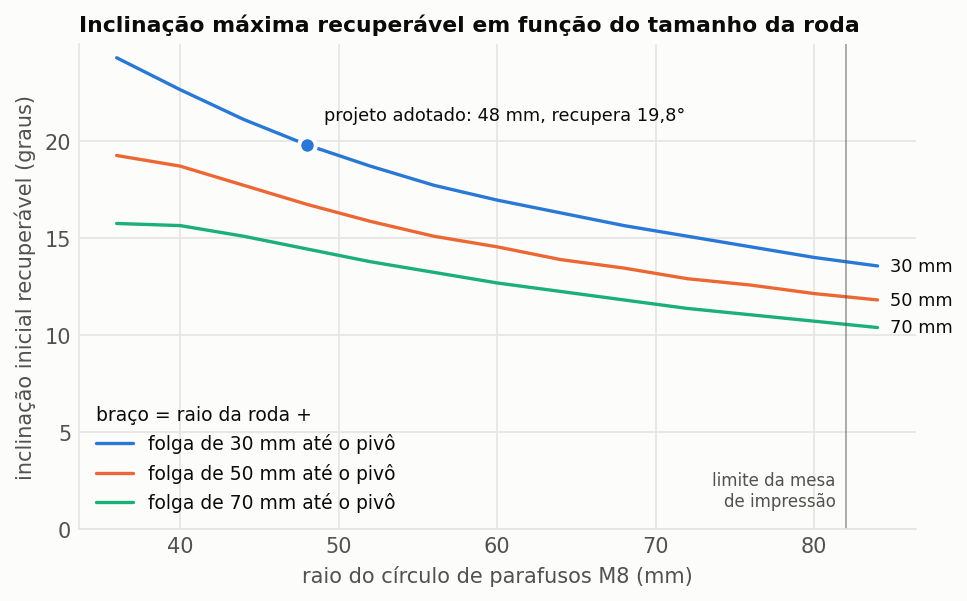
\includegraphics[width=0.82\textwidth]{dimensionamento.png}
\caption{Inclinação inicial recuperável em função do raio do círculo de parafusos, para três
folgas entre a roda e o pivô.}
\label{fig:dimensionamento}
\end{figure}

\subsection{Peças e montagem}

As peças foram modeladas em OpenSCAD, de forma paramétrica, a partir das mesmas dimensões
usadas na simulação (Figuras~\ref{fig:montagem} e~\ref{fig:pecas}). O braço gira sobre dois
rolamentos 608-ZZ numa barra de aço de \qty{8}{\milli\metre} (cortada com
\qty{\vBarraComp}{\milli\metre}), presa em dois suportes da base. Batentes inclinados de
\qty{\vAnguloBatente}{\degree}, com almofadas de TPU, limitam o curso. Os dois sensores ópticos
ficam numa prateleira sob a roda, a \qty{\vDistSensores}{\milli\metre} um do outro: uma vez e um
quarto do passo dos dentes, o que coloca os sinais em quadratura.

\begin{figure}[H]
\centering
\begin{subfigure}[b]{0.37\textwidth}\centering
  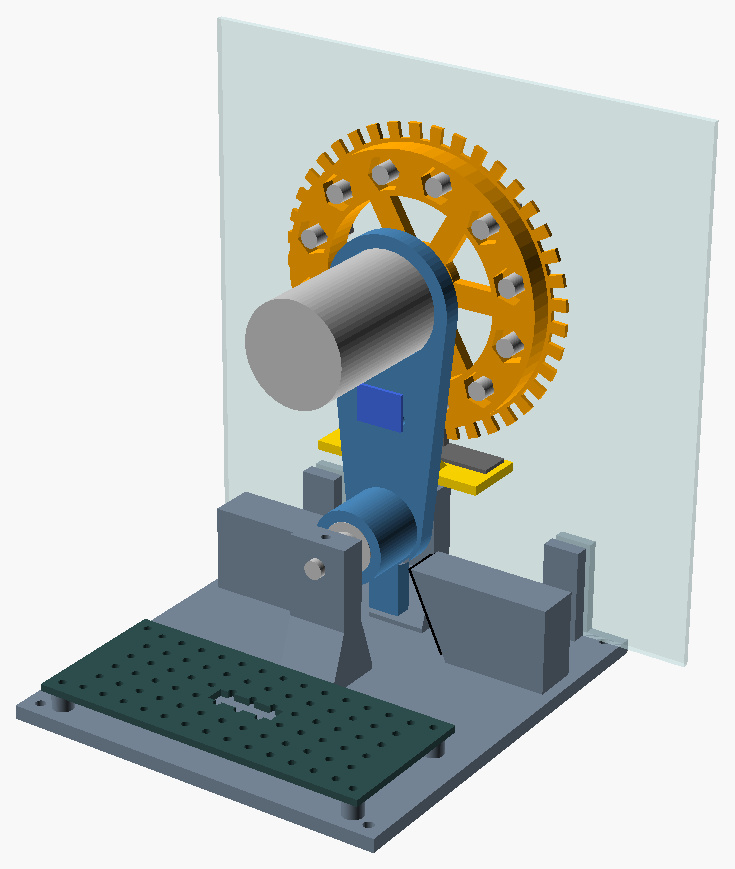
\includegraphics[width=\textwidth]{montagem_0graus_iso.png}
  \caption{Vista isométrica, com a proteção de policarbonato.}
\end{subfigure}\hfill
\begin{subfigure}[b]{0.3\textwidth}\centering
  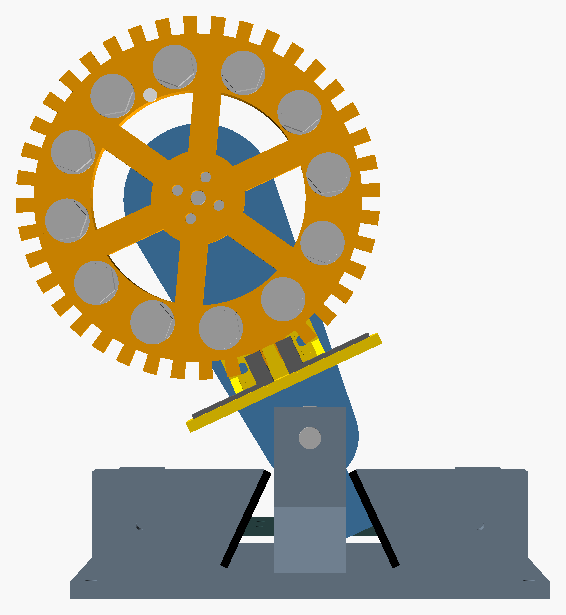
\includegraphics[width=\textwidth]{montagem_25graus_frente.png}
  \caption{Encostado no batente (\qty{\vAnguloBatente}{\degree}).}
\end{subfigure}\hfill
\begin{subfigure}[b]{0.28\textwidth}\centering
  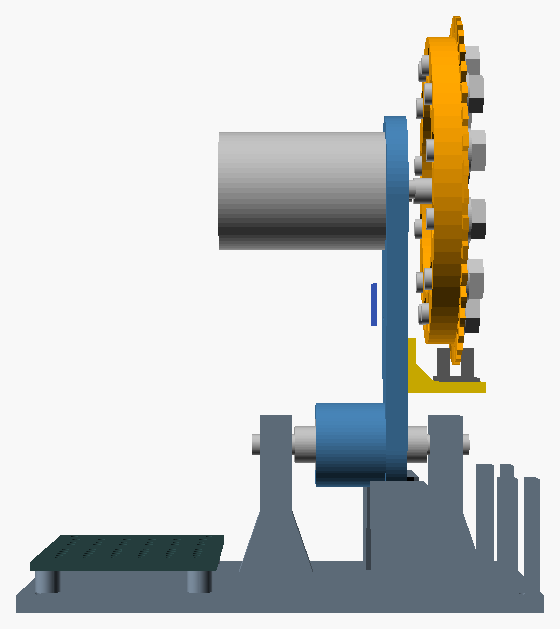
\includegraphics[width=\textwidth]{montagem_lado.png}
  \caption{Vista lateral.}
\end{subfigure}
\caption{Montagem completa gerada no OpenSCAD. Peças compradas em cinza.}
\label{fig:montagem}
\end{figure}

\begin{figure}[H]
\centering
\begin{subfigure}[b]{0.27\textwidth}\centering
  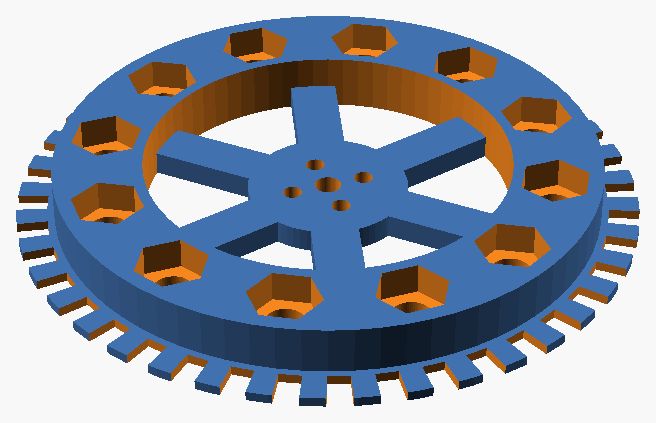
\includegraphics[width=\textwidth]{roda.png}\caption{Roda (face de trás).}
\end{subfigure}\hfill
\begin{subfigure}[b]{0.2\textwidth}\centering
  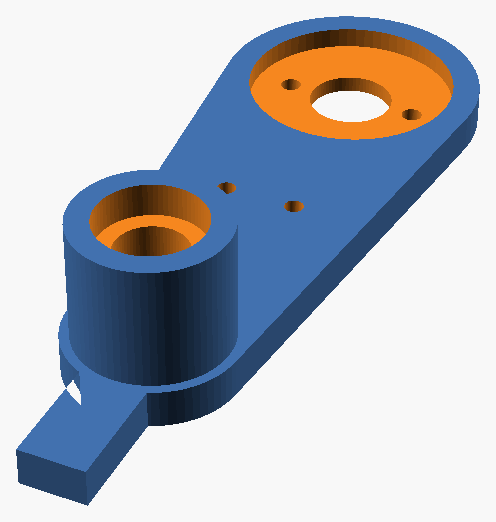
\includegraphics[width=\textwidth]{braco.png}\caption{Braço.}
\end{subfigure}\hfill
\begin{subfigure}[b]{0.25\textwidth}\centering
  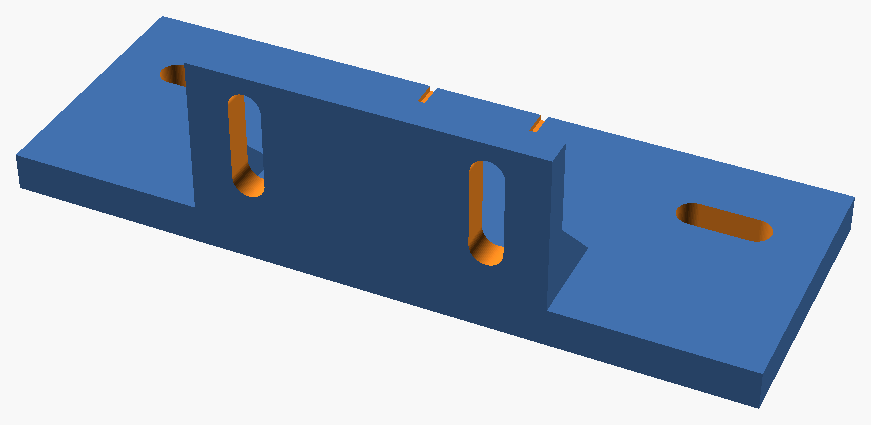
\includegraphics[width=\textwidth]{suporte_sensores.png}\caption{Suporte dos sensores.}
\end{subfigure}\hfill
\begin{subfigure}[b]{0.24\textwidth}\centering
  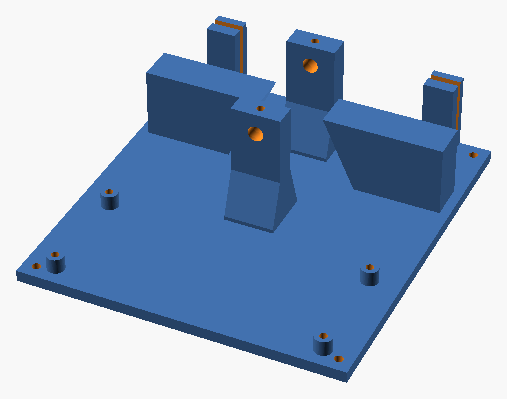
\includegraphics[width=\textwidth]{base.png}\caption{Base.}
\end{subfigure}
\caption{Principais peças impressas, na orientação de impressão (nenhuma precisa de suporte).}
\label{fig:pecas}
\end{figure}

\begin{table}[H]
\centering
\caption{Peças impressas: volume e massa calculados a partir dos STLs (PETG, com a fração de
material de cada peça).}
\label{tab:massas}
\begin{tabular}{lrrl}
\toprule
Peça & Volume (\unit{\centi\metre\cubed}) & Massa (\unit{\gram}) & Dimensões (\unit{\milli\metre}) \\
\midrule
Roda              & \num{\vCadRodaVol}            & \num{\vCadRodaMassa}            & $\vCadRodaDim$ \\
Braço             & \num{\vCadBracoVol}           & \num{\vCadBracoMassa}           & $\vCadBracoDim$ \\
Suporte dos sensores & \num{\vCadSuporteSensoresVol} & \num{\vCadSuporteSensoresMassa} & $\vCadSuporteSensoresDim$ \\
Base              & \num{\vCadBaseVol}            & \num{\vCadBaseMassa}            & $\vCadBaseDim$ \\
Bandeja da eletrônica & \num{\vCadBandejaVol}     & \num{\vCadBandejaMassa}         & $\vCadBandejaDim$ \\
Almofada de TPU (×2) & \num{\vCadBatenteTpuVol}   & \num{\vCadBatenteTpuMassa}      & $\vCadBatenteTpuDim$ \\
\bottomrule
\end{tabular}
\end{table}

A inércia da parte impressa da roda, calculada pelo STL, é
\qty{\vCadRodaInercia}{\kilo\gram\metre\squared}; somada aos parafusos e ao flange, a inércia total
usada no modelo é $I_w = \qty{\vRodaIw}{\kilo\gram\metre\squared}$. A massa do braço e a posição do
seu centro de massa usadas no modelo também vêm do CAD.

\subsection{Restrições de projeto}

Um verificador automático (\texttt{cad/folgas.py}) confere cerca de 40 folgas a cada mudança de
parâmetro, incluindo o braço girando de batente a batente. As que definiram a geometria:
\begin{itemize}
  \item o eixo do motor fica \qty{\vEixoFora}{\milli\metre} para fora do braço, o que fixa a roda a
    \qty{\vYroda}{\milli\metre} da face do braço, com o flange inteiro sobre o eixo;
  \item parafusos M8 de exatamente \qty{16}{\milli\metre}: mais compridos batem no braço;
  \item a roda precisa caber numa mesa de impressão de \qty{220}{\milli\metre};
  \item o anel dentado passa com \qty{1,5}{\milli\metre} de folga de cada lado na fenda dos sensores;
  \item a cauda do braço apoia por \qty{20}{\milli\metre} na almofada do batente, longe do tubo dos rolamentos.
\end{itemize}
Na rotação máxima permitida pelo firmware (\qty{\vWmaxRpm}{\rpm}), cada conjunto M8 puxa a borda
com \qty{\vRodaForcaParaf}{\newton} de força centrífuga, absorvida no plano das camadas de impressão.

% =====================================================================
\section{Hardware e ligações}
\label{sec:hardware}

\begin{table}[H]
\centering
\caption{Principais componentes.}
\label{tab:componentes}
\begin{tabularx}{\textwidth}{lX}
\toprule
Componente & Função \\
\midrule
WeAct Black Pill STM32F411CEU6 & controle a \qty{\vFs}{\hertz}, Cortex-M4 com FPU a \qty{96}{\mega\hertz} \\
MPU6050 (GY-521) & ângulo e velocidade angular do braço, por I2C \\
2 sensores ópticos de fenda (LM393) & encoder em quadratura da roda, \vRodaCpr{} contagens por volta \\
Ponte H BTS7960 (IBT-2) & aciona o motor nos dois sentidos, até \qty{43}{\ampere} \\
Motor CC 775, \qty{12}{\volt} & atuador; \qty{\vMotorNzero}{\rpm} em vazio (estimado) \\
Fonte \qty{12}{\volt}, \qty{10}{\ampere} + conversor buck \qty{5}{\volt} & potência do motor e da lógica \\
Fusível \qty{10}{\ampere}, TVS e capacitores & proteção do barramento \\
ST-Link V2 e adaptador USB-serial \qty{3,3}{\volt} & gravação, depuração e telemetria \\
Rolamentos 608-ZZ, barra de aço \qty{8}{\milli\metre}, colares SCC8 & pivô \\
\bottomrule
\end{tabularx}
\end{table}

\subsection{Alimentação}

\begin{figure}[H]
\centering
\begin{tikzpicture}[
  bloco/.style={draw, rounded corners=2pt, align=center, minimum height=9mm, font=\small, fill=white},
  seta/.style={-{Latex[length=2.2mm]}, thick},
  node distance=6mm and 9mm]
  \node[bloco] (f) {Fonte\\\qty{12}{\volt}};
  \node[bloco, right=of f] (fu) {Fusível\\\qty{10}{\ampere}};
  \node[bloco, right=of fu] (ibt) {IBT-2\\B+ / B$-$};
  \node[bloco, right=of ibt] (m) {Motor\\775};
  \node[bloco, below=of fu, xshift=14mm] (bk) {Buck\\\qty{5,0}{\volt}};
  \node[bloco, right=of bk, fill=blue!6] (bp) {Black Pill\\pino 5V};
  \node[bloco, above=of ibt, xshift=5mm, font=\scriptsize] (cap) {2×\qty{4700}{\micro\farad} + \qty{100}{\nano\farad}\\+ TVS SMBJ15A};
  \node[bloco, above=of fu, xshift=-10mm, font=\scriptsize] (div) {divisor \qty{10}{\kilo\ohm} / \qty{2,2}{\kilo\ohm}\\$\to$ PA4 (tensão)};
  \draw[seta] (f) -- (fu);
  \draw[seta] (fu) -- (ibt);
  \draw[seta] (ibt) -- (m);
  \draw[seta] (fu.south) |- (bk.west);
  \draw[seta] (bk) -- (bp);
  \draw[thick] (cap.south) -- (cap.south |- ibt.north);
  \draw[seta] ($(fu.east)!0.5!(ibt.west)$) |- (div.east);
\end{tikzpicture}
\caption{Distribuição de energia. O divisor mede a tensão que chega à ponte: se ela cair (fonte
fraca ou mau contato), o firmware entra em falha.}
\label{fig:alimentacao}
\end{figure}

Toda a lógica opera em \qty{3,3}{\volt}: MPU6050, sensores ópticos e a entrada lógica do IBT-2
(cujo limiar máximo é \qty{2,15}{\volt}) são alimentados pelo regulador da Black Pill, sem
conversores de nível. O pino de \qty{5}{\volt} da placa é ligado direto ao conector USB, sem
proteção; por isso a gravação é feita pelo ST-Link e a telemetria por um adaptador serial,
e o USB da placa nunca é usado com o conversor buck ligado.

\subsection{Pinagem}

\begin{table}[H]
\centering
\caption{Pinagem da Black Pill (lida de \texttt{firmware/include/board.h}).}
\label{tab:pinos}
\small
\begin{tabularx}{\textwidth}{lXl}
\toprule
Pino & Função & Periférico \\
\midrule
\tabelaPinos
\bottomrule
\end{tabularx}
\end{table}

% =====================================================================
\section{Conclusão e próximos passos}

O modelo deduzido por Euler-Lagrange descreve o pêndulo com roda de reação com duas equações
acopladas, nas quais o torque do motor aparece só na coordenada da roda e o braço o sente como
reação. Linearizado em torno do equilíbrio e escrito em variáveis de erro, o sistema é instável
mas controlável, e o LQR discreto a \qty{\vFs}{\hertz} o estabiliza com polos bem amortecidos,
recuperando o braço de até \qty{\vThetaMax}{\degree} com os limites reais de tensão e corrente.

Os parâmetros do motor ainda são estimativas: o anúncio do motor 775 informa só a faixa de
rotação. Os próximos passos são:
\begin{enumerate}
  \item medir a resistência do motor e identificar $k_e$, o atrito e $I_w$ com ensaios em patamares
    de tensão;
  \item identificar $Mgl/J$ e o atrito do pivô pela oscilação livre do braço pendurado;
  \item recalcular $K$ com os parâmetros medidos e comparar a resposta experimental com a simulada.
\end{enumerate}

% =====================================================================
\appendix
\section{Parâmetros do modelo}
\label{ap:parametros}

\begin{table}[H]
\centering
\caption{Parâmetros usados neste relatório. ``Estimado'': valor típico, a medir na bancada;
``CAD'': calculado a partir das peças modeladas; ``projeto'': escolha de projeto.}
\small
\begin{tabular}{llrl}
\toprule
Símbolo & Descrição & Valor & Origem \\
\midrule
$R$ & resistência de armadura & \qty{\vMotorR}{\ohm} & estimado \\
$L$ & indutância de armadura & \qty{\vMotorL}{\milli\henry} & estimado \\
$\omega_0$ & rotação em vazio a \qty{12}{\volt} & \qty{\vMotorNzero}{\rpm} & estimado \\
$i_0$ & corrente em vazio & \qty{\vMotorIzero}{\ampere} & estimado \\
$k_t = k_e$ & constantes de torque e de f.c.e.m. & \qty{\vMotorKe}{\newton\metre\per\ampere} & de $R$, $\omega_0$, $i_0$ \\
$\tau_c$ & atrito seco do motor & \qty{\vMotorTauC}{\milli\newton\metre} & de $i_0$ \\
$b$ & atrito viscoso do motor & \qty{\vMotorB}{\newton\metre\second\per\radian} & de $i_0$ \\
$b_{\text{eq}}$ & atrito equivalente (linearizado) & \qty{\vMotorBeq}{\newton\metre\second\per\radian} & de $i_0$ \\
$J_{\text{rotor}}$ & inércia do rotor & \qty{\vMotorJ}{\kilo\gram\metre\squared} & estimado \\
$m_m$ & massa do motor & \qty{\vMotorMassa}{\gram} & estimado \\
\midrule
$m_{\text{M8}}$ & conjunto parafuso + porca + arruela & \qty{\vRodaMconj}{\gram} & estimado \\
$r_p$ & raio do círculo de parafusos & \qty{\vRodaRparaf}{\milli\metre} & projeto \\
$m_w$ & massa da roda completa & \qty{\vRodaMassa}{\gram} & CAD + estimado \\
$I_w$ & inércia da roda + rotor & \qty{\vRodaIw}{\kilo\gram\metre\squared} & CAD + estimado \\
\midrule
$l_w$ & pivô até o eixo do motor & \qty{\vLw}{\milli\metre} & projeto \\
$m_b$ & braço com rolamentos & \qty{\vMbraco}{\gram} & CAD \\
$l_{cb}/l_w$ & posição do centro de massa do braço & \num{\vFracCm} & CAD \\
$m_e$, $l_e$ & sensores e fiação, altura & \qty{\vMextras}{\gram}, \qty{\vLextras}{\milli\metre} & estimado \\
$J$ & inércia em torno do pivô & \qty{\vJ}{\kilo\gram\metre\squared} & calculado \\
$Mgl$ & coeficiente do torque gravitacional & \qty{\vMgl}{\newton\metre} & calculado \\
$b_p$ & atrito do pivô & \qty{\vBp}{\newton\metre\second\per\radian} & estimado \\
\midrule
$V_{\text{bus}}$ & tensão da fonte & \qty{\vVbus}{\volt} & projeto \\
$u_{\max}$ & tensão máxima no motor & \qty{\vUmax}{\volt} & projeto \\
$i_{\max}$ & limite de corrente & \qty{\vImax}{\ampere} & projeto \\
$\omega_{\text{lim}}$ & limite de rotação da roda & \qty{\vWmaxRpm}{\rpm} & projeto \\
$T_s$ & período de amostragem & \qty{\vTs}{\milli\second} & projeto \\
\bottomrule
\end{tabular}
\end{table}

% =====================================================================
\begin{thebibliography}{9}
\bibitem{block}
D.~J. Block, K.~J. Åström e M.~W. Spong.
\emph{The Reaction Wheel Pendulum}.
Synthesis Lectures on Control and Mechatronics. Morgan \& Claypool, 2007.

\bibitem{ogata}
K.~Ogata.
\emph{Engenharia de Controle Moderno}. 5.\textsuperscript{a} ed. Pearson, 2010.

\bibitem{franklin}
G.~F. Franklin, J.~D. Powell e M.~L. Workman.
\emph{Digital Control of Dynamic Systems}. 3.\textsuperscript{a} ed. Addison-Wesley, 1998.

\bibitem{anderson}
B.~D.~O. Anderson e J.~B. Moore.
\emph{Optimal Control: Linear Quadratic Methods}. Prentice Hall, 1990.

\bibitem{bryson}
A.~E. Bryson e Y.-C. Ho.
\emph{Applied Optimal Control}. Hemisphere, 1975.

\bibitem{goldstein}
H.~Goldstein, C.~Poole e J.~Safko.
\emph{Classical Mechanics}. 3.\textsuperscript{a} ed. Addison-Wesley, 2002.
\end{thebibliography}

\end{document}
